\section{Multi-channel data}

In this study an ultrasound (US) dataset channel data acquired from \href{www.medicalimagingcenter.be/}{MIRC} \footnote{Medical Imaging Research Center UZ Leuven} has been utilized. The goal is to remove the US artefact and filter out the undesired part of the signal. US probe a part from the noisy contaminated signal introduces some DC level as well as low frequency signal at the onset of the time course. This appear in the US image as noise and limit the usability of this method in the near field. Additionally \textbf{\textit{wgn}} is also superimposed in the signal which needs to be removed. The US probe being used has a bandwidth from 2-7 MHz meaning that anything appearing outside this bad is considered to be noise or artefact. In this application EDS is the underlying model to be employed for subspace signal processing. Since the artefact component appear at lower frequencies with significantly higher level compare to the component sitting at the desired bad (DB) (2-7 MHz) figure \ref{US1} it is critically important to remove this component without affecting the rest of the signal. This approach would enable a much better noise suppression. 

Hereby the subspace framework is utilized wherein 28 component are computed. Then the component where their respective frequency sits outside the DB will be deduced from the original signal. The outcome from this is quite on an acceptable range, since the component of the DB sits at high values compare to the rest of the components \ref{US2}. The original and the artefact removed signal in time domain are plotted in figure \ref{UST1} and \ref{UST2} respectively.


\begin{figure}[!htbp]
\minipage{0.5\textwidth}%
\centering
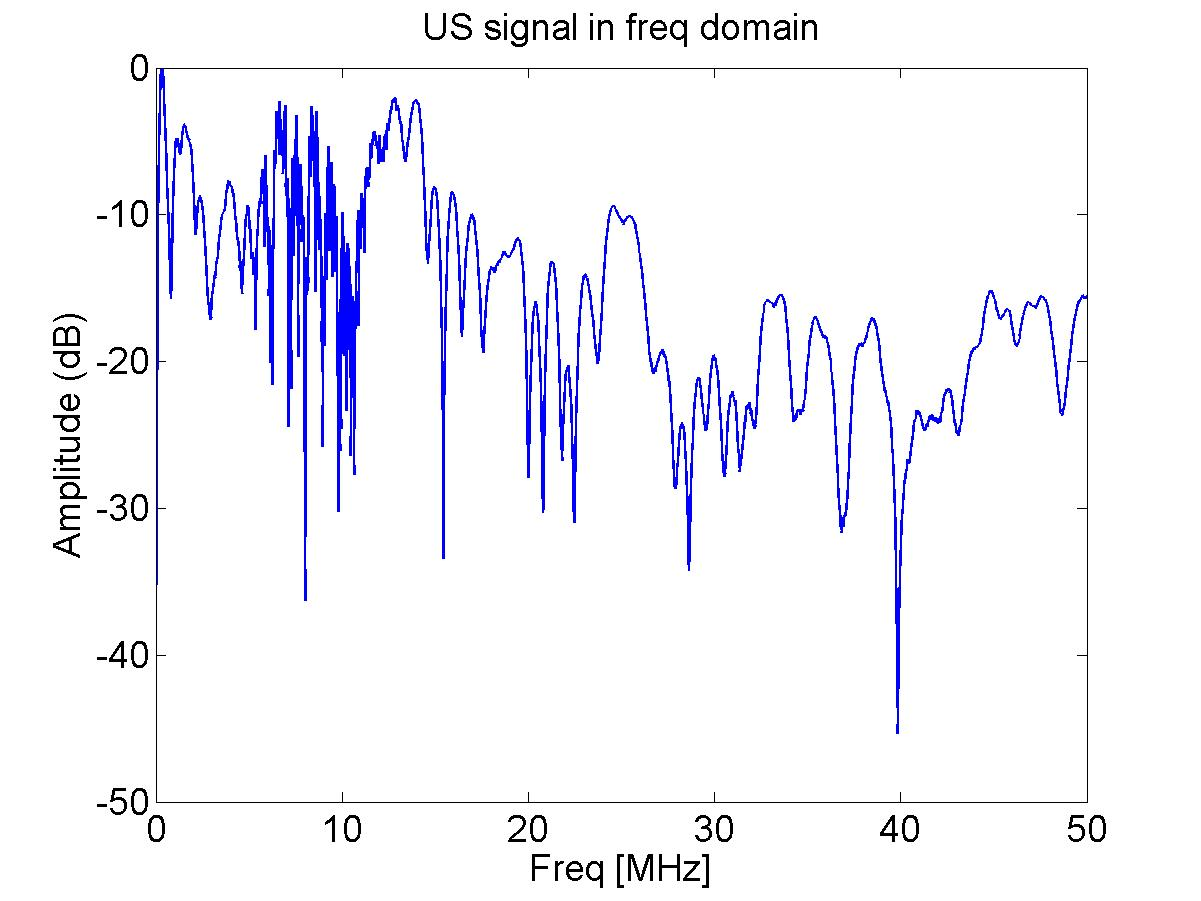
\includegraphics[width=1\textwidth]{800.jpg}
\subcaption{Original signal}\label{US1}
\endminipage\hfill
\minipage{0.5\textwidth}%
\centering
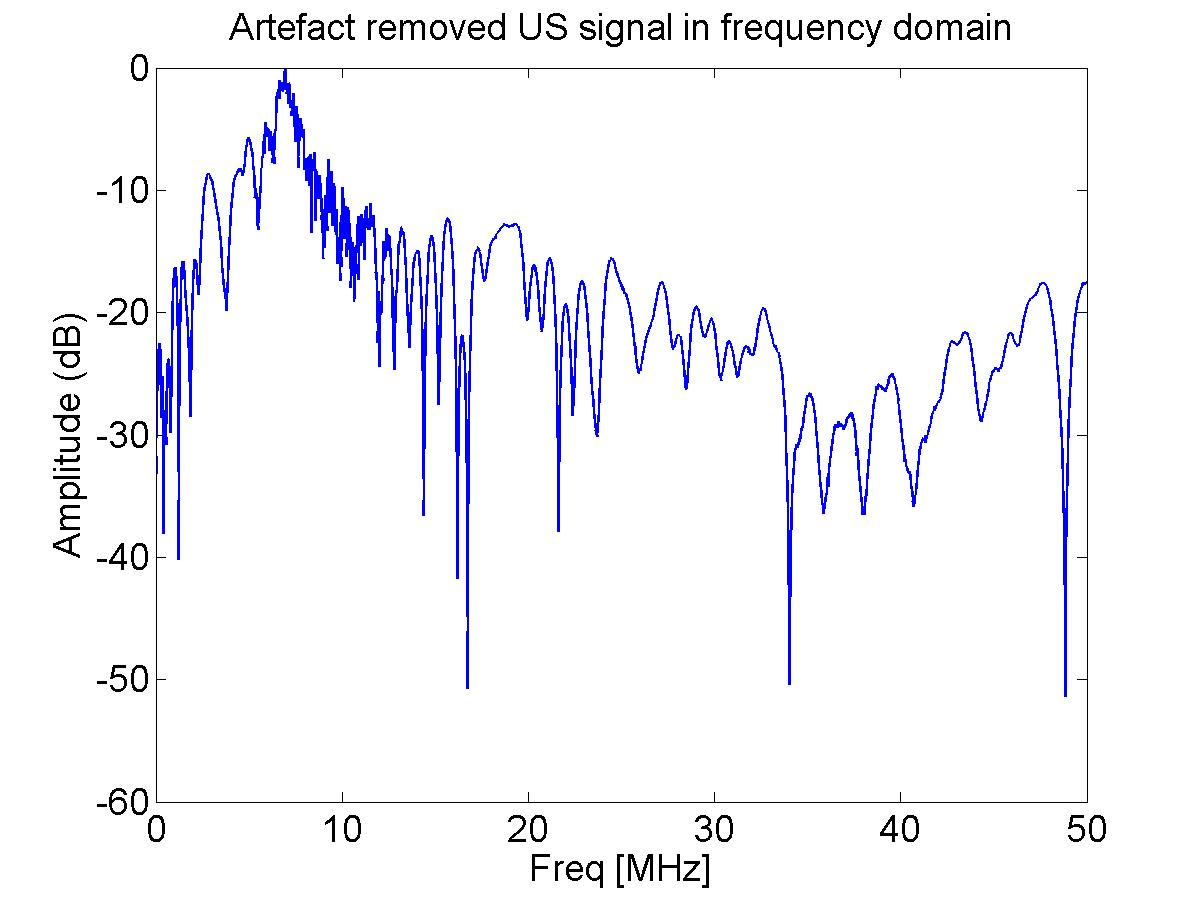
\includegraphics[width=1\textwidth]{801.jpg}
\subcaption{Artefact removed signal}\label{US2}
\endminipage\hfill
\caption{US signals.}
\end{figure}

After completing the artefact removal, signal has to be filtered out via subspace signal processing methods. Single channel algorithm Cadzow and minimum variance are alternative solution however their performance would not be the same as compare to the multichannel version of Cadzow. Single channel would not get into account the common dynamics of the of neighbouring region of interest being scanned as well as the cross talk between neighbouring ultrasound transducers inside the probe. The only drawback associated with multichannel is its time complexity increases significantly as the number of data-points is much higher. Nevertheless this could be a powerful approach for imaging stationary data via echo whereby an increase in image resolution could be achieved. 
 




\begin{figure}[!htbp]
\centering
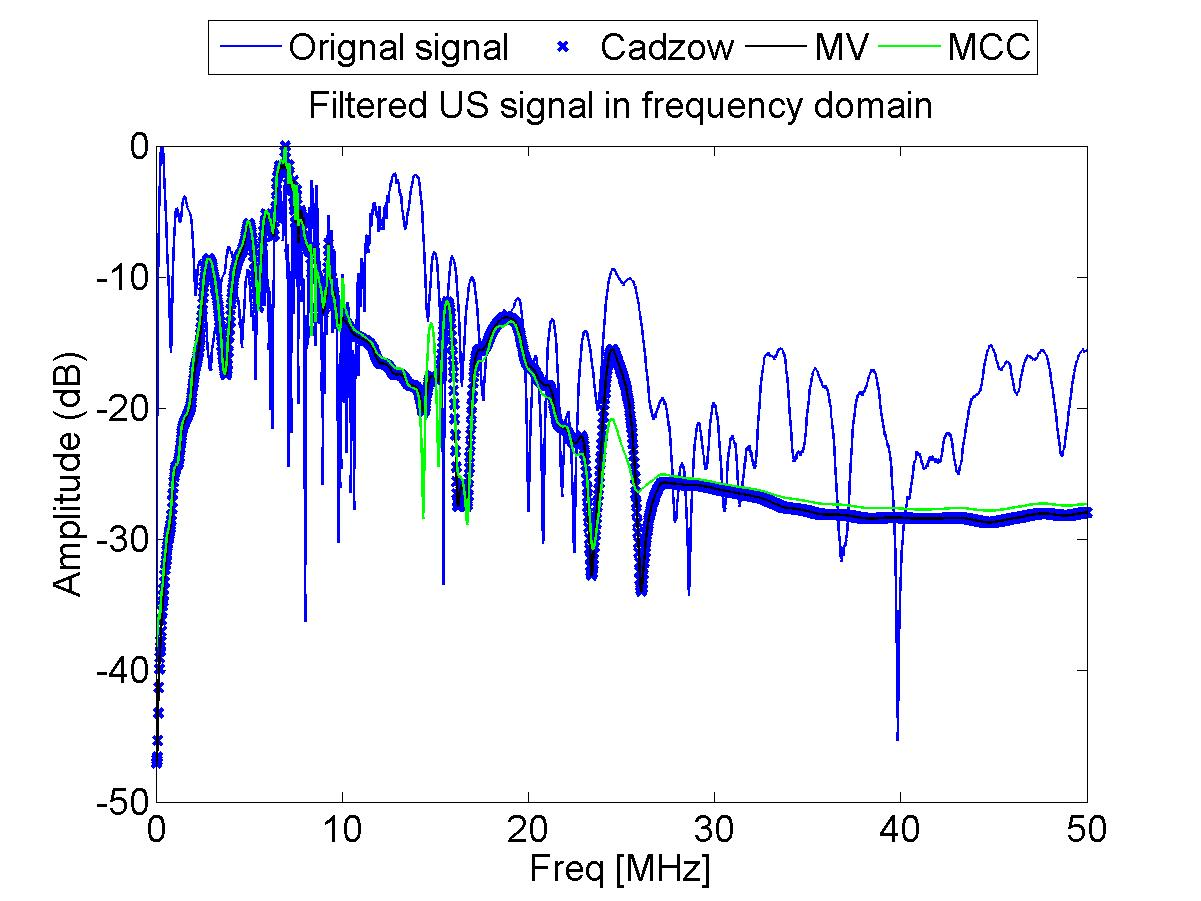
\includegraphics[width=1\textwidth]{802.jpg}
\caption{US filtered signal}\label{US3}
\end{figure}


Since subspace signal processing is a parametric method, component number of the decomposition is the only input required for this underlying model. In this case, 28 components are chosen to be sufficient number since a higher value would not yield significantly better outcome, given the time complexity would increases dramatically. 

Multichannel version would thereby overcome both this obstacles and the outperform both Cadzow and minimum variance. The filtered signal in frequency domain are overlapped in figure \ref{US3} where their respective time domain time course could be found in figure \ref{UST3},\ref{UST4},\ref{UST5}.In figure \ref{US3} are the normalised spectrum where at first glance the the filtering method suppresses the undesired spectrum down to -20 dB whereby the DB is totally untouched. 

\begin{table}[!htbp]
\centering
\caption{SNR evaluation for different methods}\label{tab12}
\begin{tabular}{c c c c c c} 
\hline 
$ $&$Original Signal$&$Cadzow$&$MV$&$MCC$ \\\hline 
            
$SNR$&$ -5.2161 $&$ 10.3109 $&$ 10.3109  $&$ 10.7620$\\
\hline 
\end{tabular}
\end{table}

In order to testify the performance of these filtering method the SNR has been computed via equation \ref{SNR1} in the frequency domain. The numerator is the variance of the DB whereas the denominator is the variance of all the components outside the DB. In table \ref{tab12} are the SNR listed where it could be increase of signal quality where the multichannel case outperforms the rest of the methods. Quite important to mention that high dynamics of the signal (very high frequency components) being filtered out via multichannel is visually notable in figure \ref{US3}.

